\documentclass[xcolor={dvipsnames}, aspectratio=169]{beamer}
\usepackage[utf8]{inputenc}
\usepackage[T1]{fontenc}
\usepackage[english]{babel}
\usetheme{Northeastern}
\usepackage{booktabs}
\usepackage{amsmath}
\usepackage{amssymb}
\usepackage{caption}
\usepackage{subcaption}
\usepackage{cancel}
\usepackage{algorithm}
\usepackage[noend]{algpseudocode}
\usepackage{standalone}
\graphicspath{{media}, {images}}
\usepackage{pgfkeys}
\usepackage[most]{tcolorbox}
\tcbuselibrary{minted}
\usepackage{codebox}

% NU colors
% from https://brand.northeastern.edu/visual-design/color/
\definecolor{NURed}{RGB}{200, 16, 46}
\definecolor{NUGold}{RGB}{164, 128, 74}
\definecolor{NUOrange001}{RGB}{255,175,128}
\definecolor{NUOrange002}{RGB}{255,153,102}
\definecolor{NUOrange003}{RGB}{255,133,79}
\definecolor{NUOrange004}{RGB}{229,98,28}
\definecolor{NUOrange005}{RGB}{187,65,0}
\definecolor{NUYellow001}{RGB}{255,255,165}
\definecolor{NUYellow002}{RGB}{255,213,128}
\definecolor{NUYellow003}{RGB}{255,196,75}
\definecolor{NUYellow004}{RGB}{255,184,56}
\definecolor{NUYellow005}{RGB}{226,168,85}
\definecolor{NUGreen001}{RGB}{189,233,201}
\definecolor{NUGreen002}{RGB}{152,209,181}
\definecolor{NUGreen003}{RGB}{96,159,128}
\definecolor{NUGreen004}{RGB}{2,89,68}
\definecolor{NUGreen005}{RGB}{26,69,56}
\definecolor{NUBlue001}{RGB}{198,239,252}
\definecolor{NUBlue002}{RGB}{160,224,239}
\definecolor{NUBlue003}{RGB}{98,182,208}
\definecolor{NUBlue004}{RGB}{43,116,150}
\definecolor{NUBlue005}{RGB}{12,51,84}

% Define colors outside of the scope of beamer themes
\newcommand{\defaultcolorheading}{NUGreen003}

% highlighted 'headings'
\newcommand{\colorheading}[1]{\textcolor{\defaultcolorheading}{\LARGE #1}}
\newcommand{\colorcaption}[1]{\textcolor{\defaultcolorheading}{\footnotesize #1}}

% Section frame, no table of contents displayed
\newcommand{\sectionframe}[2]{
  {
    \setbeamercolor{background canvas}{bg=white}
    \begin{frame}[noframenumbering, plain]
      \begin{minipage}{0.475\textwidth}
        \centering
        {\usebeamerfont{titlelike}\usebeamercolor[fg]{structure}\huge #1}
      \end{minipage}
      \hfill
      \begin{minipage}{0.45\textwidth}
        \centering
        {#2}
      \end{minipage}
    \end{frame}
  }
}

% Section frame with table of contents
\newcommand{\sectioncontentsframe}[2]{
  {
    \setbeamercolor{background canvas}{bg=white}
    \begin{frame}[noframenumbering, plain]
      \begin{center}
      \begin{minipage}{0.475\textwidth}
        \centering
        {\usebeamerfont{titlelike}\usebeamercolor[fg]{structure}\huge #1}
        \vskip2em
        \setbeamercolor{normal text}{fg=black}
        \setbeamertemplate{subsection in toc}{\leavevmode\leftskip=1.2em$\bullet$\hskip0.25em\inserttocsubsection\par}
        \tableofcontents[currentsection, sectionstyle=hide, subsubsectionstyle=hide]
      \end{minipage}
      \hfill
      \begin{minipage}{0.475\textwidth}
        \centering
        {#2}
      \end{minipage}
      \end{center}
    \end{frame}
  }
}

\newtcolorbox{alertbox}[1][]{enhanced,
  before skip=2mm,after skip=3mm,
  boxrule=0.4pt,left=5mm,right=2mm,top=1mm,bottom=1mm,
  colback=NUYellow001,
  colframe=NUYellow003,
  sharp corners,rounded corners=southeast,arc is angular,arc=3mm,
  underlay={%
    \path[fill=NUYellow005] ([yshift=3mm]interior.south east)--++(-0.4,-0.1)--++(0.1,-0.2);
    \path[draw=tcbcolframe,shorten <=-0.05mm,shorten >=-0.05mm] ([yshift=3mm]interior.south east)--++(-0.4,-0.1)--++(0.1,-0.2);
    \path[fill=NUYellow005,draw=none] (interior.south west) rectangle node[white]{\Huge\bfseries !} ([xshift=4mm]interior.north west);
  },
  drop fuzzy shadow,#1}

\newtcolorbox{infobox}[1][]{enhanced,
  before skip=2mm,after skip=3mm,
  boxrule=0.4pt,left=5mm,right=2mm,top=1mm,bottom=1mm,
  colback=NUGreen001,
  colframe=NUGreen003,
  sharp corners,rounded corners=southeast,arc is angular,arc=3mm,
  underlay={%
    \path[fill=NUGreen003] ([yshift=3mm]interior.south east)--++(-0.4,-0.1)--++(0.1,-0.2);
    \path[draw=tcbcolframe,shorten <=-0.05mm,shorten >=-0.05mm] ([yshift=3mm]interior.south east)--++(-0.4,-0.1)--++(0.1,-0.2);
    \path[fill=NUGreen003,draw=none] (interior.south west) rectangle node[white]{\Huge\bfseries i} ([xshift=4mm]interior.north west);
  },
  drop fuzzy shadow,#1}

% Pygments theme
\newcommand{\PygmentsStyle}{colorful}

% default color for boxes
\newcommand{\CodeBoxFgColor}{NUGreen005}
\newcommand{\CodeBoxBgColor}{NUGreen001!10}
\newcommand{\CodeHighlightColor}{NUOrange004!20}

% Boxes to display code
\newtcblisting[auto counter]{codeboxtc}[4]{%
  title=#2,
  listing only,
  %minted style=\PygmentsStyle,
  minted language=#1,
  boxsep=0.25mm,
  left=1mm,
  right=1mm,
  top=1mm,
  bottom=1mm,
  colback=\CodeBoxBgColor,
  colbacktitle=\CodeBoxFgColor,
  colframe=\CodeBoxFgColor,
  fonttitle=\scriptsize,
  minted options={autogobble,fontsize=\small, fontfamily=courier,
    breaklines=true, linenos, #4},
  #3
}

\newtcbinputlisting[auto counter]{\codeinput}[5]{%
  title=#2,
  listing only,
  %minted style=\PygmentsStyle,
  minted language=#1,
  boxsep=0.25mm,
  left=1mm,
  right=1mm,
  top=1mm,
  bottom=1mm,
  colback=\CodeBoxBgColor,
  colbacktitle=\CodeBoxFgColor,
  colframe=\CodeBoxFgColor,
  fonttitle=\scriptsize,
  minted options={autogobble,fontsize=\small, fontfamily=courier,
    breaklines=true, highlightcolor=\CodeHighlightColor, linenos, highlightlines=#4},
  listing file=#5,
  #3
}

\newcommand{\BeamerShowCode}[3]{%
  \pgfkeys{
    /highlight lines/.initial=4,
    /highlight lines/.get=\codehighlight,
    /highlight lines/.store in=\codehighlight,
    /extra tcb options/.initial=\empty,
    /listing file/.initial=file.cpp,
    /minipage width/.initial=1.0\textwidth,
    /box scale/.initial=1,
    /language/.initial=cpp,
  }
  \pgfkeys{#1}
  \scalebox{\pgfkeysvalueof{/box scale}}{
    \begin{minipage}{\pgfkeysvalueof{/minipage width}}
      \centering
      \codeinput{\pgfkeysvalueof{/language}}{#2}
          {\pgfkeysvalueof{/extra tcb options}}{#3}{\pgfkeysvalueof{/listing
          file}}
    \end{minipage}%
  }
}
\graphicspath{{media}, {images}}
\titlegraphic{
\includegraphics[width=0.4\paperwidth]{northeastern}}

\title{Navigating Programming Education in AI Age}
\author{Gunar Schirner, Fatema Nafa, Muhammad Salman}
\institute{Embedded Systems Laboratory (ESL)\\
  Electrical And Computer Engineering\\
  Northeastern University\\
  Boston MA, USA}
\newcommand{\footername}{AI in Programming Education}

\begin{document}

\begin{frame}[plain]
  \titlepage
\end{frame}

\begin{frame}{Outline}
  \tableofcontents[part=1]
  \tableofcontents[hideallsubsections, part=2]
  \tableofcontents[hideallsubsections, part=3]
  \tableofcontents[hideallsubsections, part=4]
  \tableofcontents[hideallsubsections, part=5]
\end{frame}

\part[Introduction]{Introduction}
\section{Introduction}

\begin{frame}{Workshop Overview}
  \begin{itemize}
    \item Workshop designed for instructors teaching programming-oriented courses
    \item Explore how AI shifts focus from syntax to system design
    \item Learn about intentional development and collaborative project management
    \item Explore different levels of AI assistance through interactive demos
    \item Translate experiences into impactful classroom practices
  \end{itemize}
\end{frame}

\begin{frame}{Workshop Objectives}
  By the end of this workshop, participants will:
  \begin{itemize}
    \item Gain understanding of AI's evolving role in programming education
    \item Explore multiple levels of AI programming assistance
    \item Gain hands-on experience with AI tools in a programming context
    \item Start designing classroom activities that meaningfully integrate AI
    \item Reflect on pedagogical shifts from coding mechanics to design thinking
  \end{itemize}
\end{frame}

\begin{frame}{Workshop Logistics}
  \begin{itemize}
    \item \textbf{Duration:} 1 hour
    \item \textbf{Target Audience:} Instructors of programming-oriented courses
    \item \textbf{Format:} Interactive, hands-on
    \item \textbf{Requirements:} 
      \begin{itemize}
        \item Basic familiarity with programming concepts
        \item A laptop for participating in activities
        \item (Optional) Access to GitHub Copilot, Claude
      \end{itemize}
  \end{itemize}
\end{frame}

\begin{frame}{Workshop Agenda}
  \begin{itemize}
    \item Overview of AI in programming education [10 minutes]
    \item Exploration of AI programming assistance levels [15 minutes]
    \item Hands-on activity design [20 minutes]
    \item Show \& Tell / Discussion [15 minutes]
  \end{itemize}
\end{frame}

\section{Increasing Abstraction in Programming}

\begin{frame}{Evolution of Programming Abstractions}
  \begin{itemize}
    \item Programming has always moved toward higher levels of abstraction
    \item Historical progression:
      \begin{itemize}
        \item Machine code → Assembly → C/C++ → Python → Domain-specific languages
      \end{itemize}
    \item Higher abstractions enable developing more complex systems with less code
    \item Focus shifts from implementation details to system design
    \item With each new abstraction level, initial concerns about:
      \begin{itemize}
        \item Performance
        \item Loss of control over implementation details
      \end{itemize}
  \end{itemize}
\end{frame}

\begin{frame}{Dominance of Higher Abstractions}
  \begin{itemize}
    \item Higher abstractions eventually dominate as compiler/runtime systems improve
    \item Example: Assembly now used only for utmost performance-critical code
      \begin{itemize}
        \item Where human expertise exceeds compiler optimization
        \item To access very specific hardware features
      \end{itemize}
    \item With Generative AI, natural language becomes a new abstraction level
    \item Allows specifying what a program should do without syntax constraints
  \end{itemize}
\end{frame}

\begin{frame}{Paradigm Shift in Programming}
  \begin{itemize}
    \item GenAI becomes peer programmer (collaborator), not just a tool
    \item Helps with:
      \begin{itemize}
        \item Generating simple scripts with a few sentences
        \item Reviewing, analyzing, and suggesting improvements
        \item Code completion, repeating, and expanding code patterns
        \item Developing complete projects across multiple files
      \end{itemize}
    \item Libraries and APIs become more accessible
    \item Single developer can span many more programming languages
  \end{itemize}
\end{frame}

\begin{frame}{Limitations of GenAI}
  \begin{itemize}
    \item GenAI is not a replacement for human programmers
    \item Still driven by human creativity, intuition, experience, and problem-solving
    \item Limited to what it abstracted from training data
    \item AI cannot build your custom, novel, high-impact project for you
    \item Can help build it faster and with less effort
    \item Helps focus on system design rather than implementation details
  \end{itemize}
\end{frame}

\begin{frame}{Changing Role of a Programmer}
  \begin{itemize}
    \item Focus shifts from \textbf{syntax and implementation mechanics} to \textbf{design, clear vision and intent}
    \item From \textbf{individual contributor} to \textbf{project team lead} where AI is a \textbf{collaborative team member}
    \item Enables larger-scale, impactful projects through AI assistance
    \item Still needs to understand the entire stack to evaluate suggestions and spot issues
  \end{itemize}
  
  \begin{alertbox}
    Comparison with aircraft autopilot:
    \begin{itemize}
      \item Autopilot helps with low-level tasks, but pilot remains in control
      \item Pilot must understand entire aircraft systems to spot and fix issues
    \end{itemize}
  \end{alertbox}
\end{frame}

\begin{frame}{Key Question}
  \begin{center}
    \large\textbf{How do we guide students in programming education to become technology leaders, while still ensuring they understand the underlying technology details?}
  \end{center}
\end{frame}

\part[AI Programming Assistance]{AI Programming Assistance}
\section{Overview of Assistance Levels}

\begin{frame}{Four Levels of AI Programming Assistance}
  We'll explore four examples of AI programming assistance, with increasing complexity and integration:
  
  \begin{enumerate}
    \item \textbf{Auxiliary Code Generation}\\
    One-shot generation of scripts beyond course focus
    
    \item \textbf{Code Review and Improvement}\\
    Analyze, debug, and enhance existing code with AI
    
    \item \textbf{Copilot Integration in VS Code}\\
    Contextual code completion with GitHub Copilot
    
    \item \textbf{Agent Mode for Complex Projects}\\
    Agentic AI systems for larger, multi-file codebases
  \end{enumerate}
\end{frame}

\section{Level 1: Auxiliary Code Generation}

\begin{frame}{Auxiliary Code Generation: Concept}
  \begin{itemize}
    \item Using AI (Claude, ChatGPT) to generate complete, functional scripts
    \item Applications: data analysis, visualization, processing
    \item Helps tackle complex coding tasks that require significant manual effort
    \item Especially useful for tasks outside the main course focus
  \end{itemize}
\end{frame}

\begin{frame}{Pedagogical Framing: Auxiliary Code}
  \begin{itemize}
    \item Courses focus on in-depth topics requiring full attention
    \item Real-world problems often require complex analysis and reasoning
    \item Not enough time to cover out-of-domain details
    \item Opportunity: Prompt AI to generate auxiliary code for:
      \begin{itemize}
        \item Simulation code
        \item Data loaders, converters
        \item Visualizations
        \item Diagnostic utilities
      \end{itemize}
  \end{itemize}
\end{frame}

\begin{frame}{Benefits of Auxiliary Code Generation}
  \begin{itemize}
    \item Students can focus on primary course objectives
    \item Analyze and interpret results through generated code
    \item Enables experiential learning in a larger context
    \item Reduces cognitive load from secondary implementation details
    \item More time for higher-order thinking and analysis
  \end{itemize}
\end{frame}

\begin{frame}{Example Scenario: Real-time Analysis}
  \begin{itemize}
    \item EECE4534: Linux Kernel Module development (in C)
    \item Students develop kernel module to generate PWM signals
    \item Code quality directly impacts signal quality
    \item Students need to capture and analyze to improve learning
    \item Shouldn't be burdened with implementing analysis code
  \end{itemize}
\end{frame}

\begin{frame}{Pulse Width Modulation Example}
  \begin{center}
    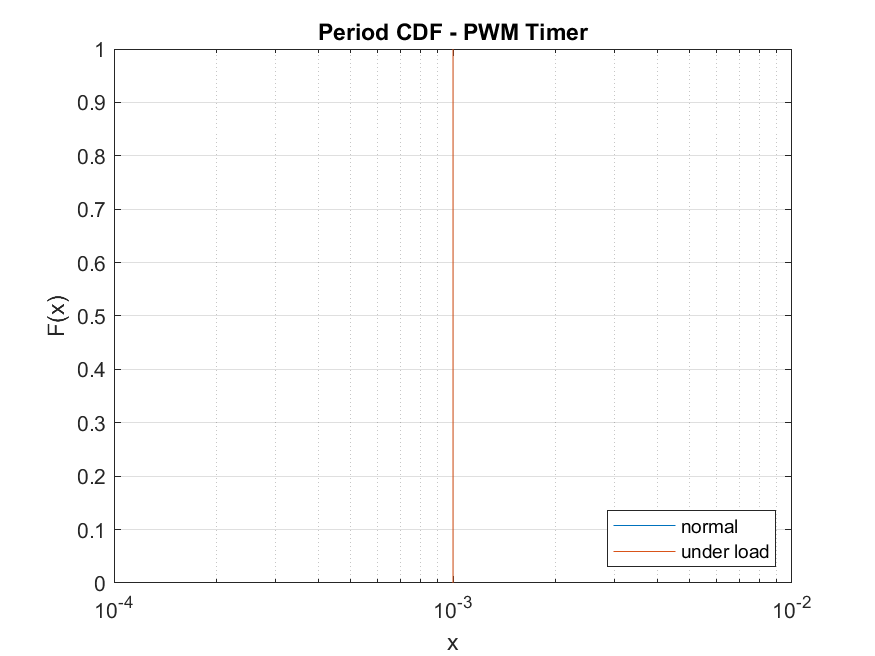
\includegraphics[width=0.6\textwidth]{/home/schirner/work/ai-prog-workshop/1-script/period_timer.png}
  \end{center}
  \begin{itemize}
    \item Hardware Timer implementation of PWM signal
    \item Empowers students to learn about their own code's performance
  \end{itemize}
\end{frame}

\begin{frame}[fragile]{Sample AI Prompt for Code Generation (1/2)}
  \begin{codeboxtc}{text}{Generated by Sonet 3.7}{}{}
"I need a Python script to analyze timing data from digital signals. I have a CSV file with the following columns:
1. Sample Time (in seconds)
2. Edge type (0 for RISING, 1 for FALLING)
3. Duration since last edge of same type (seconds)
4. Duration since last edge of opposite type (seconds)

Please write a script that:
1. Reads the CSV file
2. Extracts the latency between falling and rising edges (column 4 when edge type is 0/RISING)
  \end{codeboxtc}
\end{frame}

\begin{frame}[fragile]{Sample AI Prompt for Code Generation (2/2)}
  \begin{codeboxtc}{text}{Generated by Sonet 3.7}{}{}
3. Calculates and plots the cumulative probability distribution (CDF) of this latency
4. Adds appropriate labels, title, and grid to the plot
5. Displays some basic statistics (mean, median, min, max, standard deviation)
6. Saves the plot as a PNG file

Please include comments explaining the code and handle potential errors."
  \end{codeboxtc}
\end{frame}

\begin{frame}{Sample Output: CDF Visualization}
  \begin{center}
    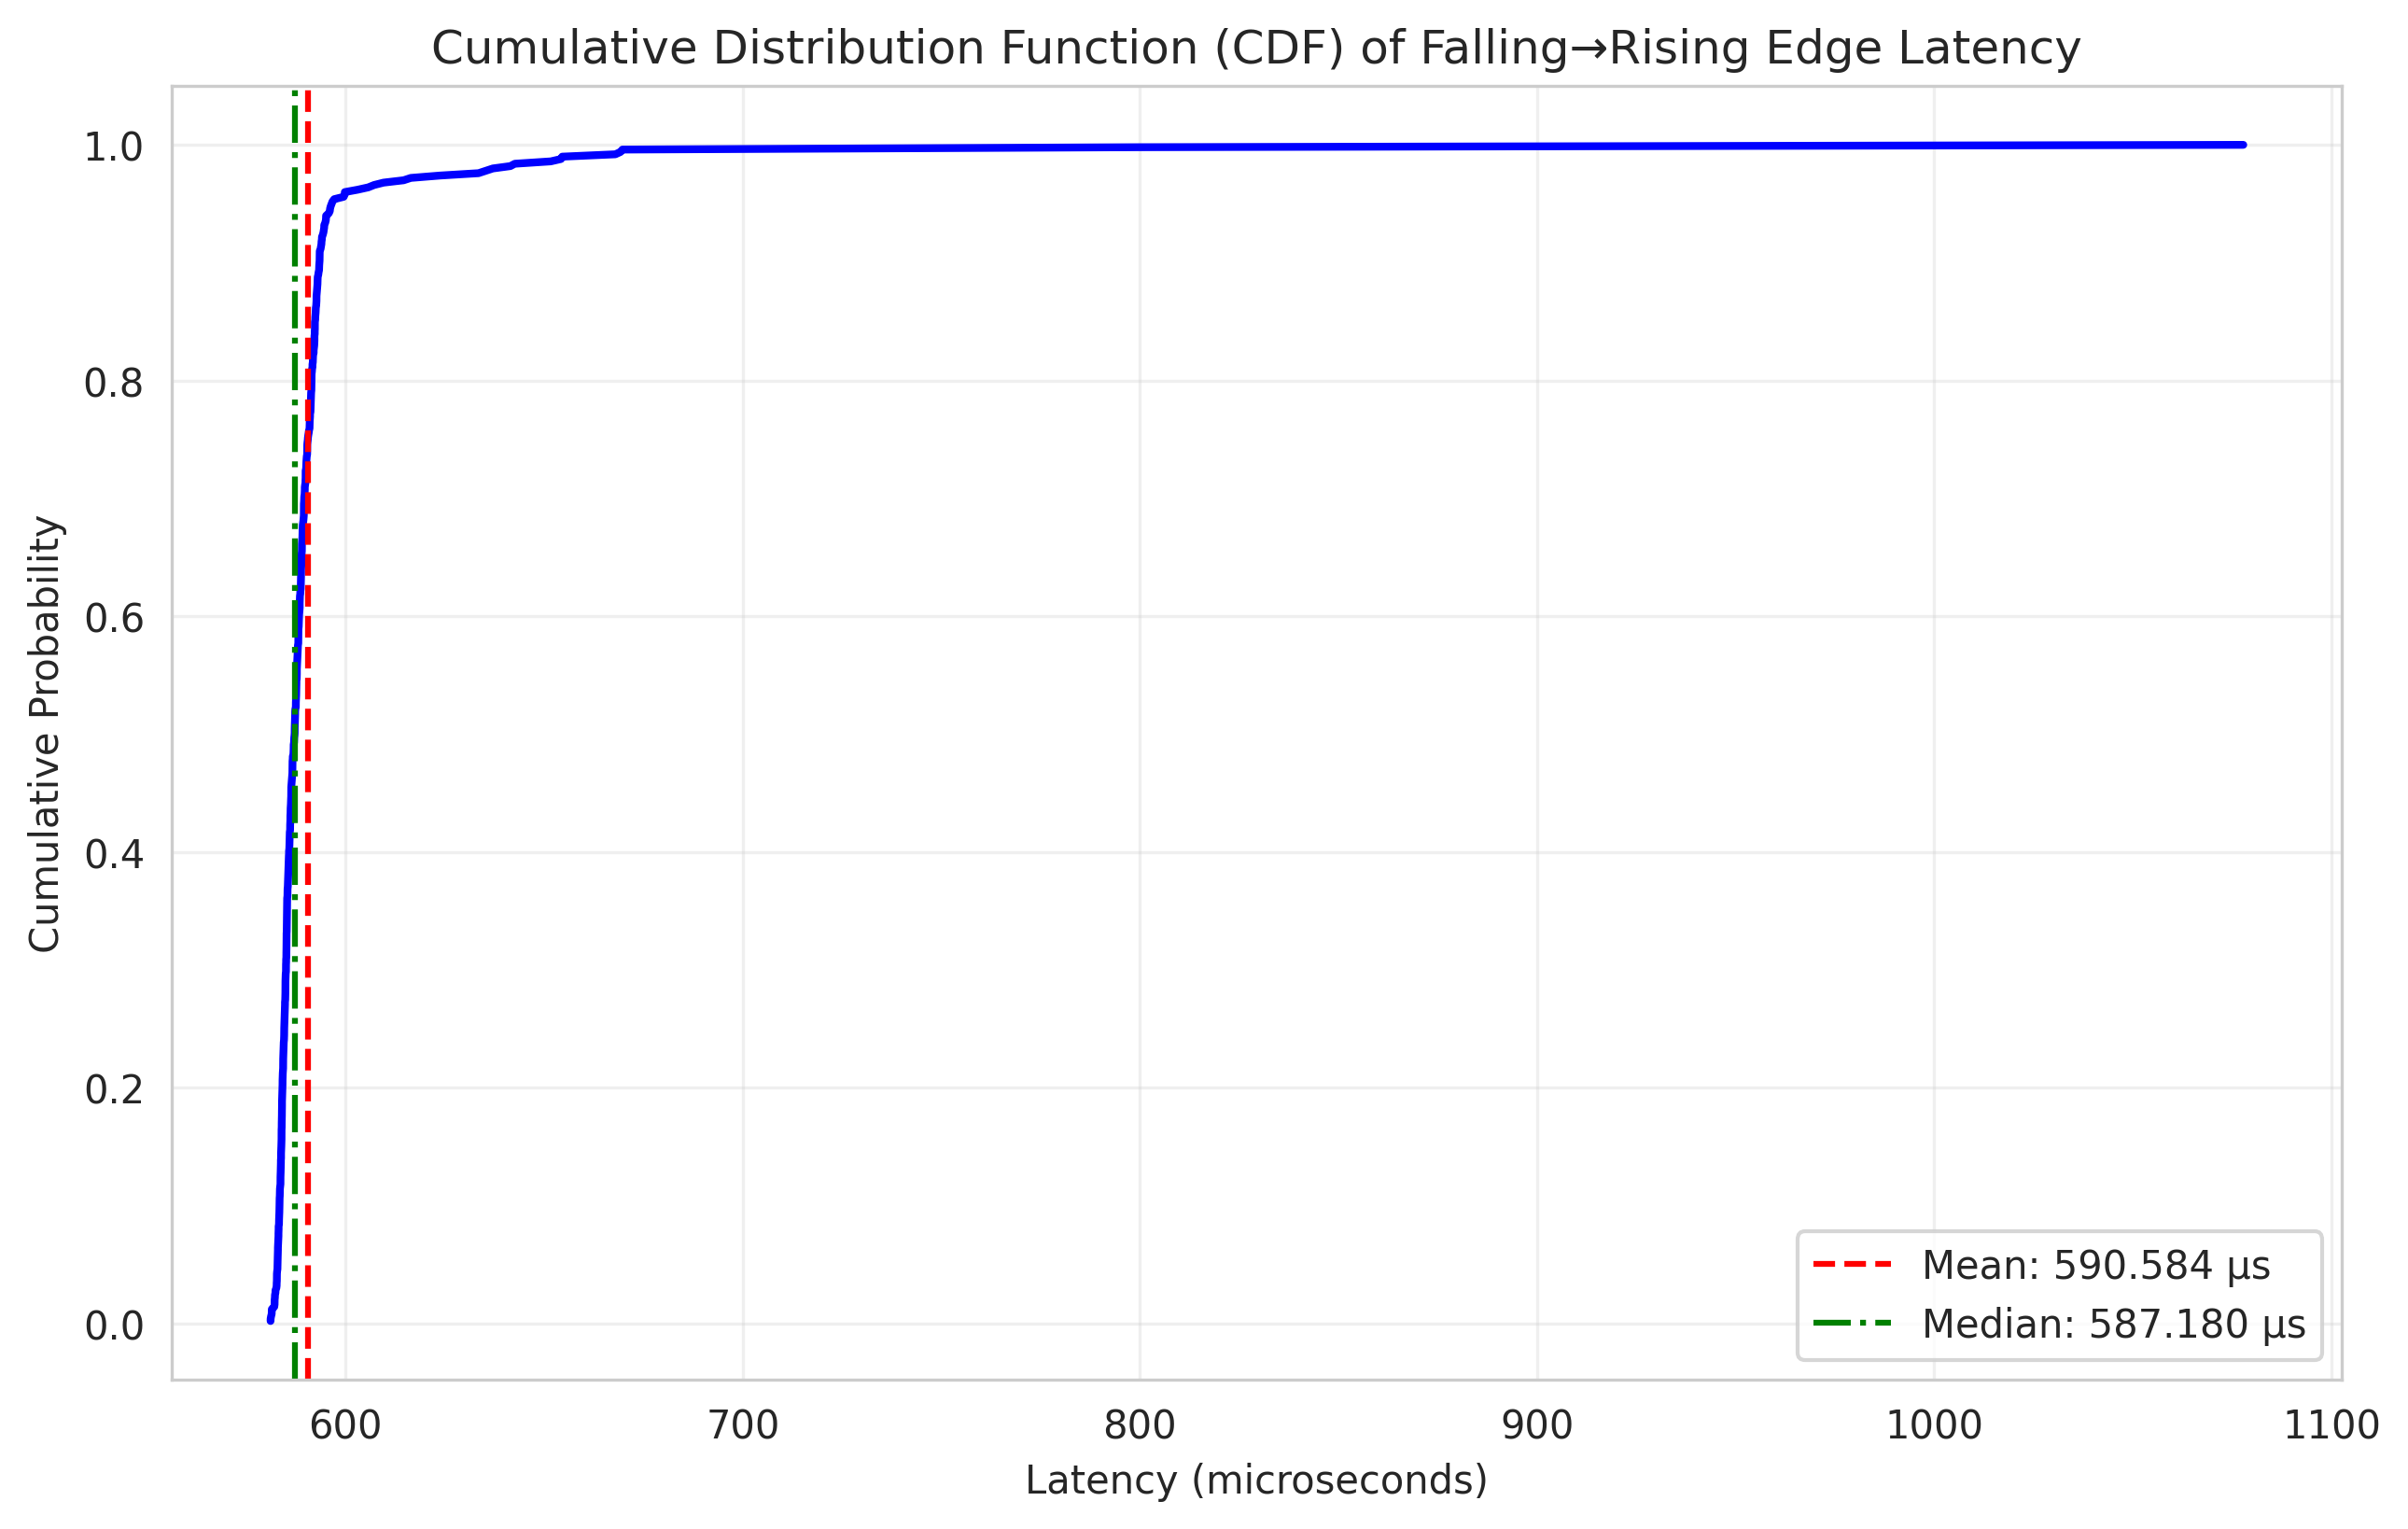
\includegraphics[width=0.7\textwidth]{/home/schirner/work/ai-prog-workshop/1-script/pwm_sleep_edges_loaded_latency_cdf.png}
  \end{center}
  \begin{itemize}
    \item Shows distribution of latencies between falling and rising edges
    \item Mean (red dashed) and median (green dash-dotted) values indicated
  \end{itemize}
\end{frame}

\begin{frame}{Instructor Activity: Auxiliary Code Generation}
  Consider how you might use this approach in your teaching:
  
  \begin{enumerate}
    \item Identify a task beyond your course scope that would enable students to focus on higher-level concepts
    \item Craft a detailed prompt for AI to generate a useful script
    \item Consider how students will learn from the enabled higher-level analysis
    \item Plan for assessment focused on understanding and interpretation rather than implementation
  \end{enumerate}
  
  This allows students to engage with more complex analyses while developing their understanding of core programming concepts.
\end{frame}

\section{Level 2: Code Review and Improvement}

\begin{frame}{Code Review and Improvement: Concept}
  \begin{itemize}
    \item Using AI as a coach to review, debug, and improve existing code
    \item Goal: Support student learning through hint-driven feedback
    \item Focuses on error identification and code optimization
    \item Provides guidance without directly giving away answers
  \end{itemize}
\end{frame}

\begin{frame}{Pedagogical Framing: Code Review}
  The goal is not to let AI do the thinking for students, but to:
  \begin{itemize}
    \item Scaffold their problem-solving process
    \item Encourage students to first analyze code themselves
    \item Use AI for targeted hints or explanations
    \item Have students reflect on and evaluate AI's suggestions
  \end{itemize}
  
  \begin{infobox}
    This approach promotes:
    \begin{itemize}
      \item Deeper understanding of algorithms and logic
      \item Collaborative learning through discussion of AI output
      \item A mindset of \textit{debugging as discovery}, not just fixing
    \end{itemize}
  \end{infobox}
\end{frame}

\begin{frame}[fragile]{Example: Faulty Merge Sort}
  \begin{codeboxtc}{python}{Faulty Merge Sort Implementation}{}{}
def merge_sort(arr):
    if len(arr) <= 1:
        return arr

    mid = len(arr) // 2
    left = merge_sort(arr[:mid])
    right = merge_sort(arr[mid]) 

    return merge(left, right)

def merge(left, right):
    sorted_list = []
    i = j = 0
    while i < len(left) or j < len(right):
        
        if i < len(left) and (j >= len(right) or left[i] < right[j]):
            sorted_list.append(left[i])
            i += 1
        else:
            sorted_list.append(right[j])
            j += 1

    return sorted_list
  \end{codeboxtc}
\end{frame}

\begin{frame}[fragile]{Suggested AI Prompt for Code Review}
  After students attempt to understand and debug the code themselves:
  
  \begin{codeboxtc}{text}{AI Prompt}{}{}
"Can you review the following merge sort implementation and highlight any possible errors or inefficiencies? Please explain what is wrong, suggest corrections, and explain how the code can be made more efficient and robust."
  \end{codeboxtc}
\end{frame}

\begin{frame}{Sample AI Response: Identified Issues (1/2)}
  \begin{enumerate}
    \item \textbf{Incorrect Slice in Recursive Call}
      \begin{itemize}
        \item \texttt{right = merge\_sort(arr[mid])} should be \texttt{arr[mid:]}
      \end{itemize}
    
    \item \textbf{Unsafe Loop Condition}
      \begin{itemize}
        \item \texttt{while i < len(left) or j < len(right)} should use \texttt{and} to avoid \texttt{IndexError}
      \end{itemize}
  \end{enumerate}
\end{frame}

\begin{frame}{Sample AI Response: Identified Issues (2/2)}
  \begin{enumerate}\setcounter{enumi}{2}
    \item \textbf{Missing Appending of Remaining Elements}
      \begin{itemize}
        \item Any unprocessed elements in \texttt{left} or \texttt{right} should be appended after the loop
      \end{itemize}
  \end{enumerate}
\end{frame}

\begin{frame}[fragile]{Corrected Implementation}
  \begin{codeboxtc}{python}{Corrected Merge Sort}{}{}
def merge_sort(arr):
    if len(arr) <= 1:
        return arr
    mid = len(arr) // 2
    left = merge_sort(arr[:mid])
    right = merge_sort(arr[mid:])
    return merge(left, right)

def merge(left, right):
    sorted_list = []
    i = j = 0
    while i < len(left) and j < len(right):
        if left[i] < right[j]:
            sorted_list.append(left[i])
            i += 1
        else:
            sorted_list.append(right[j])
            j += 1
    sorted_list.extend(left[i:])
    sorted_list.extend(right[j:])
    return sorted_list
  \end{codeboxtc}
\end{frame}

\begin{frame}{Reflection on AI Code Review}
  After receiving AI's response, students should reflect on:
  \begin{itemize}
    \item Did the AI catch all the subtle bugs?
    \item Do they understand \textit{why} those bugs matter?
    \item Would students benefit from hint-driven support?
    \item What did they learn from this debugging process?
  \end{itemize}
\end{frame}

\begin{frame}{Instructor Activity: Code Review}
  Design a classroom activity where students use AI as a code reviewer:
  
  \begin{itemize}
    \item \textbf{What kind of faulty code will you use?}
      \begin{itemize}
        \item Algorithm with subtle logic bugs?
        \item Object-oriented implementation with structural issues?
        \item Larger codebase with inefficient logic?
      \end{itemize}
    \item \textbf{How will students interact with the AI?}
      \begin{itemize}
        \item To request hints or partial feedback?
        \item To compare their debugging with AI suggestions?
      \end{itemize}
  \end{itemize}
\end{frame}

\section{Level 3: Copilot Integration}

\begin{frame}{Copilot Integration: Concept}
  \begin{itemize}
    \item GitHub Copilot supports students during coding with context-aware completions
    \item Can generate boilerplate code and scaffold structures from natural language
    \item Helps students engage more deeply with \textbf{design}, \textbf{testing}, and \textbf{debugging}
    \item Handles repetitive coding tasks to focus on higher-level thinking
  \end{itemize}
\end{frame}

\begin{frame}{Pedagogical Framing: Copilot}
  GitHub Copilot isn't just a shortcut—it's a design collaboration tool:
  \begin{itemize}
    \item Helps translate high-level \textbf{intent} into functional code
    \item Encourages focus on solution \textbf{design} rather than syntax
    \item Shifts emphasis from "getting code to run" to:
      \begin{itemize}
        \item \textbf{Designing} robust, readable, purposeful code
        \item Reviewing suggestions to ensure alignment with intent
        \item Making \textbf{critical decisions} about accepting, rejecting, or revising completions
      \end{itemize}
  \end{itemize}
\end{frame}

\begin{frame}{Example: Cluster Visualization}
  \begin{center}
    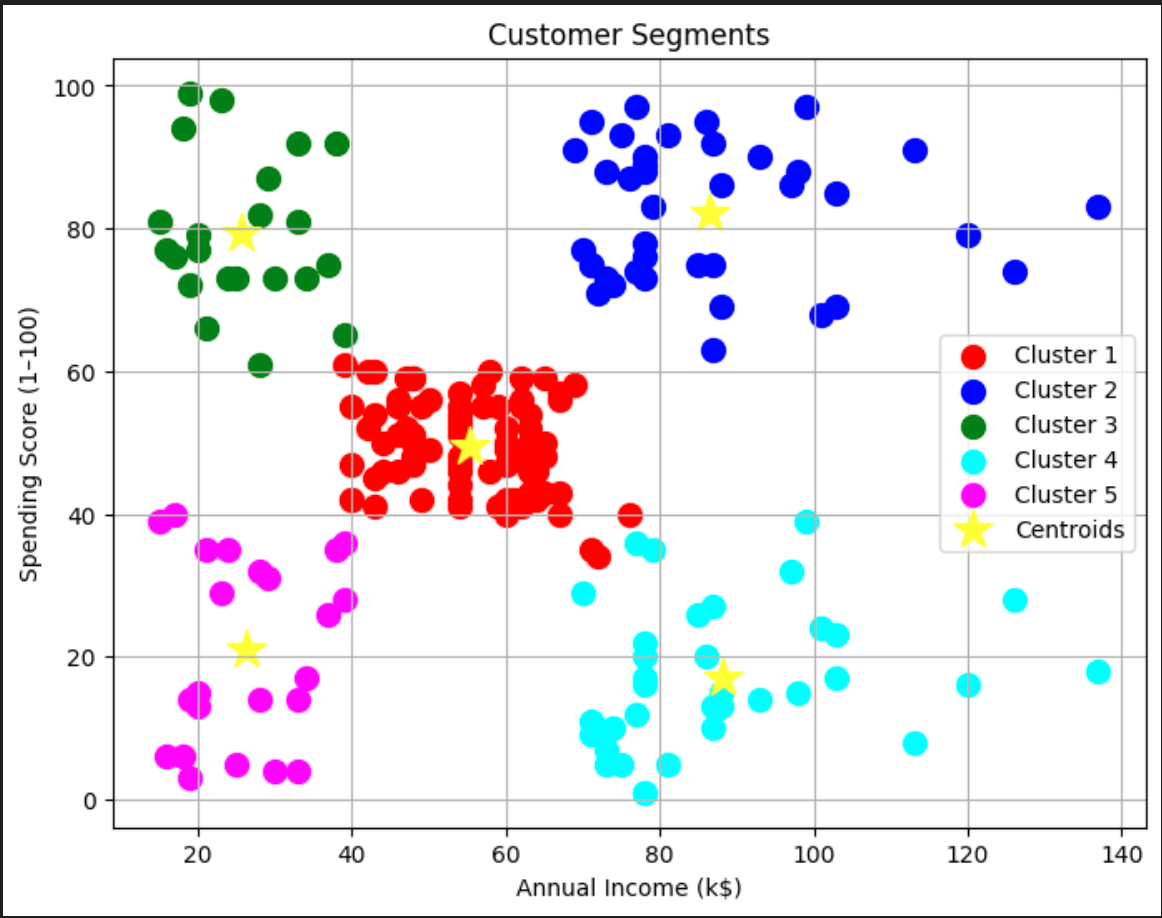
\includegraphics[width=0.6\textwidth]{/home/schirner/work/ai-prog-workshop/3-assist/Cluster.jpeg}
  \end{center}
  \begin{itemize}
    \item Scatter plot showing KMeans clustering of customers
    \item Based on annual income and spending score
    \item Students might analyze or reproduce such results
  \end{itemize}
\end{frame}

\begin{frame}{Copilot in Action}
  \begin{center}
    \textbf{[Animation showing GitHub Copilot completing code]}
  \end{center}
  \begin{itemize}
    \item Well-structured comments guide Copilot suggestions
    \item Examples of functions Copilot can generate:
      \begin{itemize}
        \item \texttt{plot\_cluster\_distribution()}
        \item \texttt{evaluate\_clustering\_quality()}
      \end{itemize}
  \end{itemize}
\end{frame}

\begin{frame}{Instructor Activity: Copilot Integration}
  Design a classroom activity where students:
  \begin{enumerate}
    \item Start from a partially written script or data processing task
    \item Use Copilot to complete functions, generate visualizations, or structure test code
    \item Reflect on how closely Copilot's output matches their original design intent
  \end{enumerate}
  
  Consider:
  \begin{itemize}
    \item What prompt would you give your students?
    \item How would you ensure critical evaluation of suggestions?
    \item Could this accelerate exploration of real-world datasets?
  \end{itemize}
\end{frame}

\section{Level 4: Agent Mode for Complex Projects}

\begin{frame}{Agent Mode: Concept}
  \begin{itemize}
    \item Using GitHub Copilot Agent Mode to tackle complex, multi-file projects
    \item Manages sophisticated projects that would be challenging in classroom contexts
    \item Helps students develop system thinking while reducing implementation overhead
    \item Enables ambitious projects that demonstrate real-world scenarios
  \end{itemize}
\end{frame}

\begin{frame}{Vibe Coding Overview}
  \begin{itemize}
    \item Focuses on rapid prototyping and collaborative iteration with AI
    \item Prioritizes agile evolution of user experience and system flow over low-level details
    \item Enables quick project scaffolding and experimentation
    \item Mainstream in startups and accelerators:
      \begin{itemize}
        \item 25\% of Y Combinator's current cohort have almost entirely AI-generated codebases
      \end{itemize}
    \item Warning: Don't over-rely on AI
  \end{itemize}
\end{frame}

\begin{frame}{Pedagogical Framing: Agent Mode}
  \begin{itemize}
    \item Experiential learning is key, involving hands-on final projects
    \item Class projects are time-constrained (4-6 weeks), limiting scope
    \item Opportunity: increase impact using Agent Mode for development
    \item Benefits:
      \begin{itemize}
        \item Students focus on system architecture and design principles
        \item Tackle more ambitious, real-world projects
        \item More experiential learning in shorter timeframe
      \end{itemize}
  \end{itemize}
\end{frame}

\begin{frame}{Challenges of Agent Mode}
  \begin{itemize}
    \item Students still need to understand the entire stack
    \item Must critically evaluate AI suggestions and spot issues
    \item Large volume of generated code can become overwhelming
    \item Need to balance convenience with learning goals
    \item Example: Accelerate AI inference with GEMM Accelerator 
      \begin{itemize}
        \item SoC and custom hardware simulation
        \item Focus on HW/SW architecture
      \end{itemize}
  \end{itemize}
\end{frame}

\begin{frame}{Example: Group Organization Tool}
  \begin{itemize}
    \item Organizing workshop participants into groups based on interests
    \item Complex web application development fast-tracked with AI
    \item Features include:
      \begin{itemize}
        \item User login (by name)
        \item Interest selection from predefined options
        \item Admin role for team formation
        \item Team assignment and display
        \item Optional team chat functionality
      \end{itemize}
  \end{itemize}
\end{frame}

\begin{frame}[fragile]{Sample Prompt for Agent Mode}
  \begin{codeboxtc}{text}{Prompt for GitHub Copilot in VS Code (Agent Mode)}{}{}
Generate a web page to which session participants can login (just by name no authentication required). After logging in, each participant needs to select from one of the following interests:
- Code Improvement and Teaching
- Code Assistance with CoPilot
- Script Generation
- Agent Mode for Projects

A coordinator (username admin) finishes the first phase (after all participants have logged in). Then participants are paired together based on interests into teams (Teams get named team-1, team-2 ...). Each team should contain 2-2 members. The participants should get their team name and team members displayed once the decision is done. Optionally, members in the tam should be able to chat with each other
  \end{codeboxtc}
\end{frame}

\begin{frame}{Instructor Activity: Agent Mode}
  Consider how you might use Agent Mode in your teaching:
  
  \begin{enumerate}
    \item Identify a complex, multi-component project that would normally be challenging to implement
    \item Draft a detailed system specification focusing on learning objectives
    \item Create a prompt template for students to use with Agent Mode
    \item Consider assessment criteria emphasizing system design, integration patterns, and architectural choices
  \end{enumerate}
  
  This approach allows students to engage with sophisticated projects while developing valuable system thinking skills.
\end{frame}

\part[Hands-on Activity]{Hands-on Activity}
\section{Activity Design}

\begin{frame}{Hands-on Activity Overview}
  Form groups of 2 based on interest in AI assistance levels:
  \begin{itemize}
    \item Preferably select a level challenging you beyond current experience
    \item Your team will be assigned a breakout room
  \end{itemize}
  
  Then:
  \begin{itemize}
    \item Explore your chosen technology level
    \item Design a classroom activity integrating AI at this level
    \item Leverage AI assistants to build your activity
    \item Prepare to share with the larger group
  \end{itemize}
  
  Time: 15 minutes
\end{frame}

\begin{frame}{Activity Design Considerations}
  When designing your activity, consider:
  \begin{itemize}
    \item Expected outcomes/skills
    \item Expressiveness and scalability of assessment
    \item How to minimize anticipated challenges
    \item Ways to foster student engagement and ownership
    \item Opportunities for deeper learning
  \end{itemize}
\end{frame}

\part[Discussion and Reflection]{Discussion and Reflection}
\section{Show \& Tell}

\begin{frame}{Share and Discuss}
  \begin{itemize}
    \item Selected groups share activity ideas, challenges, and insights
    \item Discuss implementation approaches
    \item Identify common themes and innovations
    \item Consider adaptations for different course contexts
  \end{itemize}
\end{frame}

\section{Reflection}

\begin{frame}{Impact on Learning}
  \begin{itemize}
    \item Discuss how integrating AI could impact student learning
    \item Consider ways tools might reshape assignments and course design
    \item Identify potential challenges in:
      \begin{itemize}
        \item Assessment
        \item Fairness
        \item Over-reliance on AI
      \end{itemize}
    \item Explore opportunities to foster deeper engagement and ownership
  \end{itemize}
\end{frame}

\begin{frame}{Continued Exploration}
  \begin{itemize}
    \item Too many ideas, too many changes to explore in one hour!
    \item Launchpad for ongoing discussion and collaboration
    \item Consider regular (e.g., bi-weekly) meetups to:
      \begin{itemize}
        \item Share observations, challenges, and new ideas
        \item Support each other in programming education evolution
      \end{itemize}
    \item Next step: kick-off programming community meeting
  \end{itemize}
\end{frame}

\part[Conclusion]{Conclusion}
\section{Conclusion}

\begin{frame}{Contributing \& Continuing the Conversation}
  We welcome contributions from instructors adapting these resources:
  \begin{itemize}
    \item Fork the repository and customize materials
    \item Submit issues or suggestions for improvement
    \item Add your own classroom AI integration examples
  \end{itemize}
  
  Let's build a collaborative, forward-thinking community of educators who embrace AI not as a shortcut—but as a tool for thoughtful, empowering, and meaningful learning.
\end{frame}

\begin{frame}{Acknowledgments}
  This workshop was created by:
  \begin{itemize}
    \item \href{https://coe.northeastern.edu/people/schirner-gunar/}{Gunar Schirner}
    \item \href{https://coe.northeastern.edu/people/nafa-fatema/}{Fatema Nafa}
    \item Muhammad Salman
  \end{itemize}
  
  at Northeastern University.
  
  \vspace{1em}
  
  Claude and other AI tools have been used in the process of ideation and drafting the workshop.
\end{frame}

\begin{frame}{Thank You!}
  \begin{center}
    \Large{Questions and Discussion}
    
    \vspace{2em}
    
    GitHub Repository:\\
    \texttt{https://github.com/neu-ece-esl/ai-prog-workshop}
  \end{center}
\end{frame}

\end{document}
